\documentclass[12pt]{article}
%[10pt,technote]{IEEEtran}
\usepackage{hyperref}
\usepackage{graphicx}
\usepackage[affil-it]{authblk}
\usepackage{color}
\usepackage{amsgen,amsmath,amstext,amsbsy,amsopn,amssymb}
\usepackage{geometry}
\usepackage{subcaption}
\usepackage{caption}
\usepackage{wrapfig}
\usepackage{comment}
\usepackage{mathrsfs}
\usepackage{upgreek}
\usepackage{amssymb}
\usepackage{textcomp}
\usepackage{amsmath}
\usepackage{tcolorbox}
\usepackage{listings}
\usepackage{fancyhdr}
\usepackage{cite}
\usepackage{wasysym} 
%\usepackage{subfigure}
%\usepackage{wraptable}

\geometry{left=2.5cm, right=2.5cm,top=2.5cm,bottom=2.5cm}
\makeatletter
\newcommand{\rmnum}[1]{\romannumeral #1}
\newcommand{\Rmnum}[1]{\expandafter\@slowromancap\romannumeral #1@}
\makeatother


\setcounter{secnumdepth}{0}
\title{\bf The Emergence of Monitors\\
   \large Are Monitors Beneficial for Society? }

\author{Jiani Gao\\Elisa Taveras Pena\\Iryna Anufriyeva\\Thanh Pham\\Justin Kizner}
\affil{Department of Economics, Binghamton University}
\date{\today}
\pagestyle{fancy}
\chead{} \lhead{}\rhead{}
\cfoot{jgao30@binghamton.edu}

\begin{document}
\maketitle
\newpage
%\tableofcontents	

\newpage
\noindent
\section{\Rmnum{1.} Introduction}
When determining the public policy strategy a government should adopt, a solid framework for policy analysis of complex economic systems is an essential part of the process.  An important instance of public policy to observe and implement is that of a common-pool resource (CPR). In her 2009 Nobel Prize lecture, Elinor Ostrom explores the different principles a polycentric government could use to develop a framework for institutional analysis and implementation. 

The principle we explore in this paper is Principle 4, which states the importance on Monitoring in a CPR system. It states “Individuals who are accountable to or are the users monitor the appropriation and provision levels of the users. Individuals who are accountable to or are the users monitor the condition of the resource (Ostrom, 2009).” To expand, this principle claims that agents will act in their own best interest to create a monitoring system in order to preserve the resource for a longer period of time.  

We use an agent based model to recreate the scenario of a CPR  in order to observe an emergence of monitoring. The model includes a lake with with three different fish populations, of varying values. Our model tests the longevity of the same community with and without monitoring, and then strives to observe an emergence of a stable model where individuals can alternate between monitors and fishermen based on the conditions of the fish (ie the fish population remaining in the lake) and the overall happiness of the agent.




\section{\Rmnum{2.} The Model}
To recreate the scenario of a CPR and test the effects of monitoring, we construct two models, which have very similar settings but different looks. We do analysis based on the first model.
\begin{figure}[!h]
\caption{Left: Model 1, Right: Model 2}
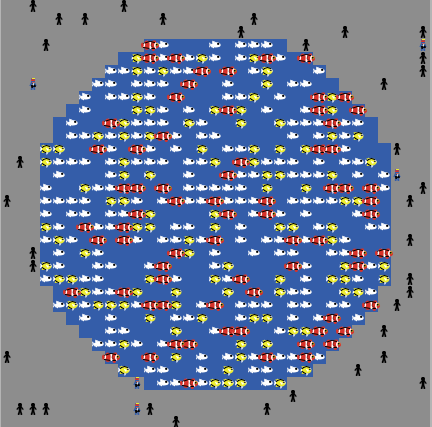
\includegraphics[width=3in,height=3in]{model1}
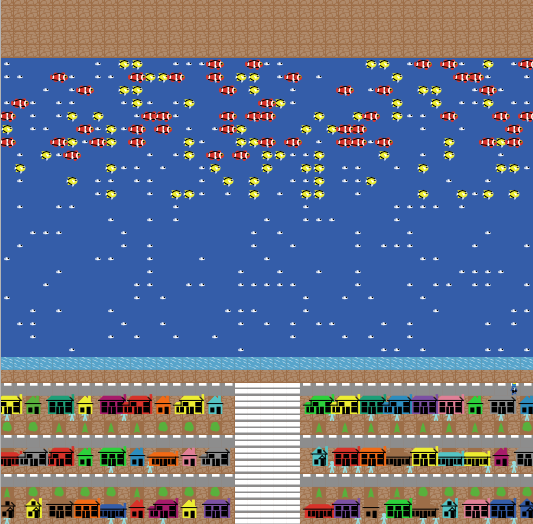
\includegraphics[width=3in,height=3in]{model2}
\end{figure}
\newpage
In our model, we have:
\begin{enumerate}
	\item Two types of agents: \textbf{fisherman} and \textbf{monitor}.
	\begin{enumerate}
		\item Fisherman
		\begin{itemize}
			\item Fishermen take fish from lake.
			\item There are 40 hours per day, fisherman go fish in the first 30 hours, and then go home to take rest.
			\item Fishermen get happiness from catching fish, and different types of fish will give them different happiness. Specifically, carp: 1 unit of happiness, salmon: 2 units of happiness, tilapia: 6 units of happiness.
			\item Chance of catching a fish per tick: similar to wolves-sheep model, people wander around and find preys.
			\item Fisherman moves out if he/she doesn't catch enough fish, unless he/she is chosen to be a monitor for next period.
			\item Each fisherman has a probability to break rules at the start of each day (catch more fish than dialy quota). 
			\item Rule breakers who get caught have to give all their fish to the monitor.
			\item If a rule breaker get caught today, he will not overfish tomorrow no matter what happens.
		\end{itemize}
		
		
		\item Monitor
		\begin{itemize}
			\item Monitors check fishermen within a certain distance every night.
			\item Monitor is set to be happy, so they will not move out. He or she takes away all happiness from rule breakers who get caught.
			\item If a monitor catches zero rule breaker, he/she will trun into a fisherman.
		\end{itemize}
	\end{enumerate}
	

   
    \item Emergence rule.
    \begin{itemize}
    	\item At the beginning, we have five monitors.
    	\item Community decides to increase the number of monitors if one of the two cases below happen:
    	\[	\left\{
    		\begin{array}{cc}
    		A.&\text{The number of fish in the lake is less than 40\% of the original lebel}\\
    		B.&\text{The number of unhappy fishermen is greater than 70\%}	
    		\end{array}
    		\right    	
    		.\]
    	\item New monitor is selected randomly from fishermen who are unhappy. (collective decision)
    	\item Community decides to turn a monitor into a fisherman, if this monitor catches zero rule breaker.  	
    \end{itemize}
    
  
    \item Fish
    \begin{itemize}
    	\item There are 3 fishes: carp, salmon, tilapia,
    	\item They reproduce at different rates.
    	\item Different types of fish have different size and values.
    \end{itemize}

    
    \item Environment.
    \begin{itemize}
    	\item One lake.
    	\item Link patches outside the lakes with agents, so everybody has a fixed location.
    \end{itemize}
    
\end{enumerate}

\section{\Rmnum{3.} Results and Analysis}
In order to test the emergence in our ABM, we ran a behavior space analysis. We tested both models for tens runs to see which community would have a higher rate of survival. 

On average, we found that without monitors, the  time a community will survive is 60.5 days. It die because the fishermen have caught all the fish without restraints, and there is no more CPR available in order to survive, or too many people overfish and a lot fishermen cannot get enought fish to sustain their minimum happiness level, so they move out. (Below result is from Bahavior Space. The raw dara can be found in the excel file: $without\_raw\_data$.)
\begin{figure}[!h]\centering
	\caption{Survive time without monitors}
	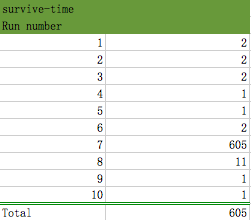
\includegraphics[width=2in,height=1.7in]{r1}
\end{figure}


However, in a model with monitoring, the average time the community will survive is 3256.5 days. This is likely the effect of increased monitoring effects when the resource begins to sharply decline in population due to overfishing, or the self interest of fishermen who have a decreased level of happiness to elect more monitors. (Below result is from Bahavior Space. The raw dara can be found in the excel file: $with\_raw\_data$.)
\begin{figure}[!h]\centering
	\caption{Survive time with monitors}
	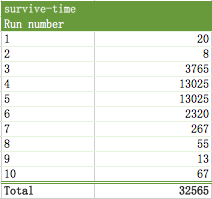
\includegraphics[width=2in,height=1.7in]{r2}
\end{figure}

Also in our model with monitoring, the number of fishermen and monitors fluctuate within a certain range. (\textit{Black line stands for fishermen and Red line stands for monitors})
\begin{figure}[!h]\centering
	\caption{Number of fishermen and monitors}
	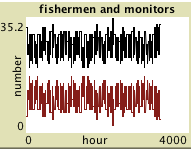
\includegraphics[width=2in,height=1.7in]{fm}
\end{figure}

We believe that it is more efficient for a community to have a system of monitoring in place since it significantly lengthens the longevity of the CPR, and creates a utility function for the agents where their happiness and actions are directly affected by the conditions of the resource. 

\section{\Rmnum{4.} Conclusion}





%\bibliographystyle{unsrt} 
%\bibliography{}
\end{document}
